\documentclass[tikz,border=10pt]{standalone}
\usepackage{amsmath}
\usetikzlibrary{arrows.meta,angles,quotes,calc}

\begin{document}
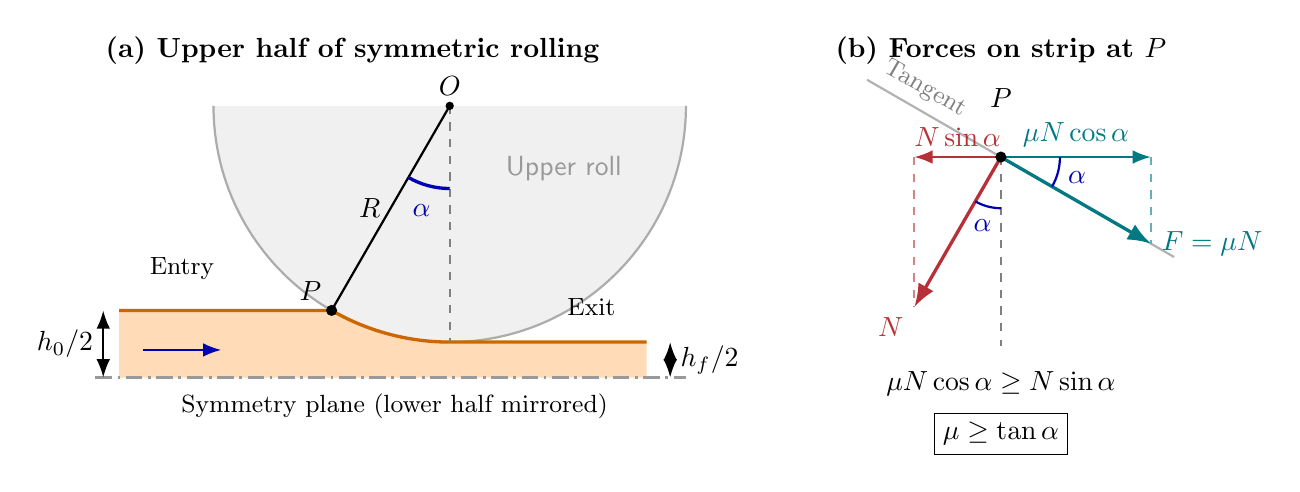
\begin{tikzpicture}[>=Latex,font=\sffamily, thick]
\definecolor{normal}{RGB}{184,48,55}
\definecolor{friction}{RGB}{0,121,131}
% Exact upper-half geometry: R=3, alpha=30 deg, hf/2=0.45.
\pgfmathsetmacro{\entry}{3.45-3*cos(30)}
\coordinate (O) at (0,3.45);
\coordinate (P) at (-1.5,\entry);
\node[anchor=west,font=\bfseries] at (-4.5,4.15) {(a) Upper half of symmetric rolling};
% Only the lower semicircle of the upper roll is needed.
\path[fill=gray!12,draw=gray!65] (-3,3.45)
 arc[start angle=180,end angle=360,radius=3];
\path[fill=orange!28] (-4.2,0)--(-4.2,\entry)--(P)
 arc[start angle=240,end angle=270,radius=3]
 --(2.5,0.45)--(2.5,0)--cycle;
\draw[orange!80!black,very thick] (-4.2,\entry)--(P)
 arc[start angle=240,end angle=270,radius=3]--(2.5,0.45);
\draw[dash pattern=on 6pt off 2pt on 1pt off 2pt,gray!80]
 (-4.5,0)--(3,0);
\node[below,font=\small] at (-0.7,-0.08) {Symmetry plane (lower half mirrored)};
\draw[<->] (-4.4,0)--(-4.4,\entry) node[midway,left] {$h_0/2$};
\draw[<->] (2.8,0)--(2.8,0.45) node[midway,right] {$h_f/2$};
\draw[dashed,gray] (O)--(0,0.45);
\draw (O)--(P) node[midway,left] {$R$};
\fill (O) circle (1.5pt) node[above] {$O$};
\fill (P) circle (2pt) node[above left] {$P$};
\draw[blue!70!black,very thick] ($(O)+(240:1.05)$)
 arc[start angle=240,end angle=270,radius=1.05];
\node[blue!70!black] at ($(O)+(255:1.38)$) {$\alpha$};
\draw[->,blue!70!black] (-3.9,0.35)--(-2.9,0.35);
\node[font=\small,above] at (-3.4,1.12) {Entry};
\node[font=\small,above] at (1.8,0.65) {Exit};
\node[gray!80] at (1.45,2.65) {Upper roll};

% Local force diagram; vector lengths are schematic.
\begin{scope}[shift={(7,2.8)}]
\node[font=\bfseries] at (0,1.35) {(b) Forces on strip at $P$};
\coordinate (Q) at (0,0);
\draw[gray!60] (-1.7,0.9815)--(2.2,-1.2702);
\node[gray,font=\small,above,rotate=-30] at (-1.1,0.635) {Tangent};
\draw[dashed,gray] (0,0)--(0,-2.4);
\draw[->,normal,very thick] (0,0)--(-1.1,-1.9053)
 node[below left] {$N$};
\draw[->,friction,very thick] (0,0)--(1.9053,-1.1)
 node[right] {$F=\mu N$};
\draw[->,normal] (0,0)--(-1.1,0) node[midway,above] {$N\sin\alpha$};
\draw[->,friction] (0,0)--(1.9053,0) node[midway,above] {$\mu N\cos\alpha$};
\draw[dashed,normal!60] (-1.1,0)--(-1.1,-1.9053);
\draw[dashed,friction!60] (1.9053,0)--(1.9053,-1.1);
\draw[blue!70!black] (-90:0.65) arc[start angle=-90,end angle=-120,radius=0.65];
\node[blue!70!black] at (-105:0.9) {$\alpha$};
\draw[blue!70!black] (-30:0.75) arc[start angle=-30,end angle=0,radius=0.75];
\node[blue!70!black] at (-15:1.0) {$\alpha$};
\fill (0,0) circle (2pt) node[above=14pt] {$P$};
\node[align=center] at (0,-3.25)
 {$\mu N\cos\alpha\ge N\sin\alpha$\\[6pt]$\boxed{\mu\ge\tan\alpha}$};
\end{scope}
\end{tikzpicture}
\end{document}
